
\documentclass[twoside]{article}
\usepackage[a4paper]{geometry}
\geometry{verbose,tmargin=2.5cm,bmargin=2cm,lmargin=2cm,rmargin=2cm}
\usepackage{fancyhdr}
\pagestyle{fancy}

\usepackage{bbm}
% nastaven� pisma a �e�tiny
\usepackage{lmodern}
\usepackage[T1]{fontenc}
\usepackage[cp1250]{inputenc}
%\usepackage[czech]{babel}	

% odkazy
\usepackage{url}

\usepackage{algorithm}
\usepackage{algorithmic}
\usepackage{bbm}

% v�cesloupcov� tabulky
\usepackage{multirow}
\usepackage{amsfonts}
% vno�en� popisky obr�zk�
\usepackage{subcaption}
\usepackage{amsmath}
% automatick� konverze EPS 
\usepackage{graphicx} 
\usepackage{epstopdf}
\usepackage{float}
% odkazy a z�lo�ky
\usepackage[unicode=true, bookmarks=true,bookmarksnumbered=true,
bookmarksopen=false, breaklinks=false,pdfborder={0 0 0},
pdfpagemode=UseNone,backref=false,colorlinks=true] {hyperref}

% Pozn�mky p�i p�ekladu
%\usepackage{xkeyval}	% Inline todonotes
%\usepackage[textsize = footnotesize]{todonotes}
%\presetkeys{todonotes}{inline}{}

% Zacni sekci slovem ukol
%\renewcommand{\thesection}{�kol \arabic{section}}
% enumerate zacina s pismenem
%\renewcommand{\theenumi}{\alph{enumi}}
\usepackage{amsmath}
\usepackage{pdflscape}
\usepackage{changepage}
\usepackage{amssymb}
\usepackage{multicol}
\usepackage{amsthm}

% smaz aktualni page layout
\fancyhf{}
% zahlavi
\usepackage{titling}
\fancyhf[HC]{\thetitle}
\fancyhf[HLE,HRO]{\theauthor}
\fancyhf[HRE,HLO]{\today}
 %zapati
\fancyhf[FLE,FRO]{\thepage}

% �daje o autorovi
\title{CVaR Q-learning Convergence - Problem Statement}
\author{Silvestr Stanko}
%\date{\today}
\setlength{\parindent}{0pt}%


%%%%%%%%%%%%%%%%%%%%%%%%%%%%%%
\usepackage{algorithm}
\usepackage{algorithmic}
\usepackage{amsthm}
\usepackage{datetime}


\newdateformat{monthyeardate}{\monthname[\THEMONTH], \THEYEAR}

\newcommand{\todo}[1]{\begingroup
            \color{Red} \textbf{todo:} {#1}
        	\endgroup }
        	
\newcommand{\unclear}[1]{\begingroup
            \color{Orange} \textbf{unclear:} {#1}
        	\endgroup }



\newcommand{\cvar}{\text{CVaR}}
\newcommand{\var}{\text{VaR}}

\newcommand{\envelope}{\mathcal{U}_{\cvar}(\alpha, P(\cdot | x, a))}



\newcommand{\indicator}{\mathbb{1}}
\renewcommand{\exp}{\mathbb{E}}
\newcommand{\expval}[1]{\mathbb{E}\left[ {#1} \right]}


%\newcommand{\exp}{\mathbb{E}}
\newcommand{\given}[1][]{\:#1\vert\:}

\newtheorem{theorem}{Theorem}
\newtheorem{corollary}{Corollary}
\newtheorem{lemma}{Lemma}



\newcommand{\bround}[1]{\left( {#1} \right)}
\newcommand{\bsquare}[1]{\left[ {#1} \right]}
\newcommand{\braces}[1]{\left{ {#1} \right}}





\begin{document}

The aim of this document is to describe the CVaR Value Iteration algorithm, it's distributional version and the extension to Q-learning. This is done in order to formulate the CVaR Q-learning convergence problem.

Let's start with some definitions.

\subsection{Return}
We define the return $Z^\pi(x)$ as a random variable representing the discounted reward along a trajectory generated by the MDP by following policy $\pi$, starting at state $x$:
\begin{equation}\label{eqn:return}
\begin{split}
&Z^\pi(x)=\sum_{t=0}^\infty \gamma^tR(x_t,a_t)\\
&x_t \sim p(\cdot|x_{t-1}, a_{t-1}), a_t \sim \pi, x_0 = x
\end{split}
\end{equation}
As a useful notation, we denote $Z^\pi(x, a)$ as the random variable representing the discounted reward along a trajectory generated by first selecting action $a$ and then following policy $\pi$.
\begin{equation}
\begin{split}
&Z^\pi(x, a)=\sum_{t=0}^\infty \gamma^tR(x_t,a_t)\\
&x_t \sim p(\cdot|x_{t-1}, a_{t-1}), a_t \sim \pi, x_0 = x, a_0 = a
\end{split}
\end{equation}

\subsection{CVaR}
Let $Z$ be a random variable representing reward, with cumulative distribution function (c.d.f.) $F(z) = \mathbb{P}(Z \le z)$.
The Value-at-Risk  at confidence level $\alpha \in (0,1)$ is the $\alpha$-quantile of $Z$, i.e. 
\begin{equation}
\text{VaR}_\alpha(Z)=F^{-1}(\alpha)=\inf\left\lbrace z | \alpha \le F(z) \right\rbrace
\end{equation}

The Conditional Value-at-Risk (CVaR) at confidence level $\alpha \in (0,1)$ is defined as the expected reward of of outcomes worse than the $\alpha$-quantile ($\var_\alpha$):
\begin{equation}\label{eqn:cvardef}
\text{CVaR}_\alpha(Z) = \dfrac{1}{\alpha}\int_0^\alpha F^{-1}_Z(\beta) \text{d}\beta = \dfrac{1}{\alpha}\int_0^\alpha \text{VaR}_\beta(Z) \text{d}\beta
\end{equation}
\cite{rockafellar2000optimization} also showed that CVaR is equivalent to the solution of
\begin{equation}\label{eqn:cvarprimal}
\text{CVaR}_\alpha(Z)=
\max_s\left\lbrace \dfrac{1}{\alpha}\expect
\left[ (Z-s)^-\right] + s  \right\rbrace 
\end{equation}
where $(x)^- = \min(x, 0)$ represents the negative part of $x$ and in the optimal point $s^* = VaR_\alpha(Z)$
\begin{equation}
\text{CVaR}_\alpha(Z)= \dfrac{1}{\alpha}\expect \left[ (Z-VaR_\alpha(Z))^-\right] + VaR_\alpha(Z)
\end{equation}
See \figref{cvardist} for a visualization.

\begin{figure}
\center
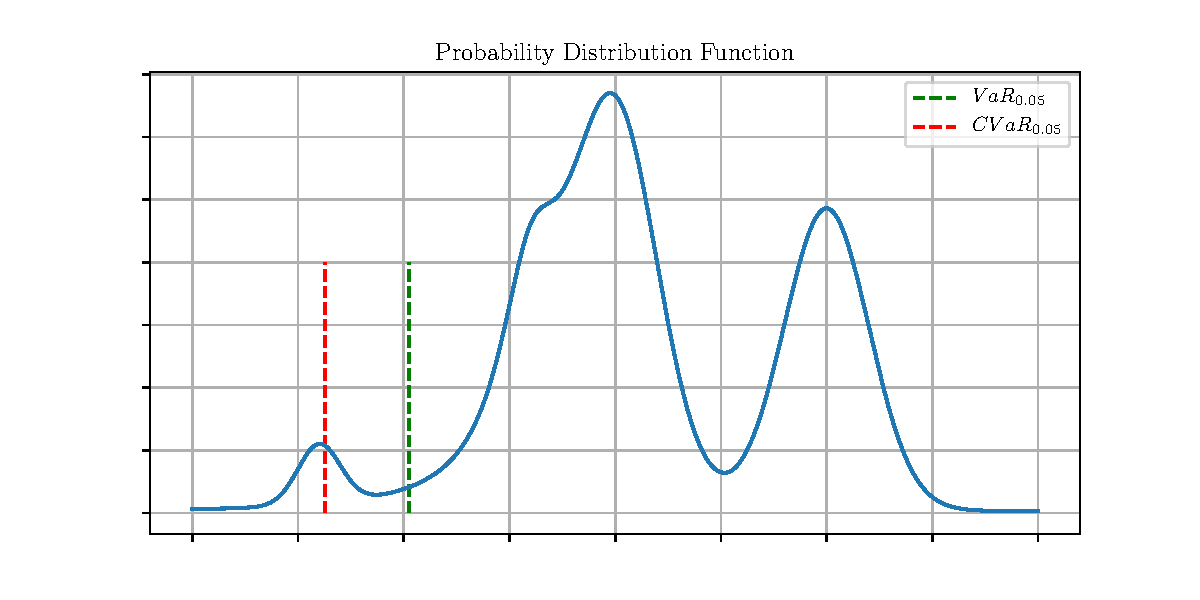
\includegraphics[width=\linewidth]{../gfx/pdf.pdf}
\caption{Value-at-Risk and Conditional Value-at-Risk of a general probability distribution with the integral $\alpha=0.05$ marked in yellow. The main flaw of the VaR metric is clearly visible here, as we could shift the leftmost 'mode' of the distribution into minus infinity and the VaR would remain unchanged, while CVaR would change with the shift.}\label{fig:cvardist}
\end{figure}

The risk-averse objective we wish to address for a given confidence level $\alpha$ is the following
\begin{equation}\label{eqn:problem}
\max_{\pi \in \Pi_H} \text{CVaR}_\alpha(Z^\pi(x_0))
\end{equation}
where $Z^\pi(x_0)$ coincides with definition \eqnref{return}.

In words, our goal is to find a general policy $\pi^*\in \Pi_H$, that maximizes conditional value-at-risk of the return, starting in state $x_0$. We emphasize the importance of the starting state since, unlike the expected value, the CVaR objective is not time-consistent.

\subsection{Value Iteration}
Value iteration \cite{sutton1998reinforcement} is a well-known algorithm for computing the optimal (action-)value function and hereby finding the optimal policy. Let us remind ourselves of the Bellman optimality operator $\cT$ \eqnref{bellmanoptimalityoperator}:
\begin{equation*}
\cT Q(x,a) := \expval{ R(x, a)} + \gamma \expect\nolimits_{P} \bsquare{\max_{a' \in \cA}Q(x', a')}
\end{equation*}
or rewritten for the value function $V$
\begin{equation}
\cT V(x) = \max_a\braces{r(x, a) + \gamma\sum_{s'}p(s'|x, a)V(x')}
\end{equation}



\section{CVaR Value Iteration}\label{sec:vi:cvar}

\cite{chow2015risk} present a dynamic programming formulation for the CVaR MDP problem \eqnref{problem}. As CVaR is a time-inconsistent measure, their method requires an extension of the state space. A Value Iteration type algorithm is then applied on this extended space and \cite{chow2015risk} proved it's convergence. 

We repeat their key ideas and results bellow, as they form a basis for our contributions presented in later sections. 

\subsection{Bellman Equation for CVaR}

The results of \cite{chow2015risk} heavily rely on the CVaR decomposition theorem (Lemma 22, \cite{pflug2016time}):
%
\begin{equation}\label{eqn:cvardecomp}
\cvar_\alpha\bround{Z^\pi(x)} = \min_{\xi \in \envelope} \sum_{x'} p(x'| x, \pi(x))\xi(x') \cvar_{\xi(x')\alpha}\bround{Z^\pi(x')}
\end{equation}
%
where $\envelope = \braces{\xi : \xi(\omega) \in \bsquare{0, \frac{1}{\alpha}}, \int_{\omega} \xi(\omega)\mathbb{P}(\omega) \text{d}\omega = 1}$.
The theorem states that we can compute the $\cvar_\alpha\bround{Z^\pi(x, a)}$ as the minimal weighted combination of $\cvar_\alpha\bround{Z^\pi(x')}$ under a probability distribution perturbed by $\xi(x')$.

Note that the decomposition requires only the representation of CVaR at different confidence levels and not the whole distribution at each level, which we might be tempted to think because of the time-inconsistency issue.

\cite{chow2015risk} extend the decomposition theorem by defining the \emph{CVaR value function} $C(x, y)$ with an augmented state-space $\mathcal{X}\times\mathcal{Y}$ where $\mathcal{Y}=(0,1]$ is an additional continuous state that represents the different confidence levels.
%
\begin{equation}\label{eqn:cdef}
C(x, y)=\max_{\pi \in \Pi_H} \cvar_{y}\bround{Z^\pi(x)}
\end{equation}
%
Similar to standard dynamic programming, it is convenient to work with with operators defined on the space of value functions. This leads to the following definition of the CVaR Bellman operator $\mathbf{T}:\mathcal{X}\times\mathcal{Y}\to\mathcal{X}\times\mathcal{Y}$:
%
\begin{equation}
\mathbf{T}C(x, y) = \max_a \bsquare{ R(x, a) + \gamma \min_{\xi \in \envelope} \sum_{x'} p(x'| x, a)\xi(x') C\bround{x', y\xi(x')}}
\end{equation}
%
or in our simplified notation, this describes the following relationship:
%
\begin{equation}\label{eqn:tcvar}
\mathbf{T} \cvar_y(Z(x))=\max_a \bsquare{R(x, a) + \gamma \cvar_{y}(Z(x, a))}
\end{equation}
%
\cite{chow2015risk} further showed (Lemma 3) that the operator $\mathbf{T}$ is a contraction and also preserves the convexity of $y \cvar_t$. The optimization problem \eqnref{cvardecomp} is a convex one and therefore has a unique solution. Additionally, the fixed point of this contraction is the optimal $C^*(x, y) = \max_{\pi \in \Pi} \cvar_y (Z^\pi(x, y))$ (\cite{chow2015risk}, Theorem 4).
 
Naive value iteration with operator $\mathbf{T}$ is unfortunately unusable in practice, as the state space is continuous in $y$. The solution proposed in \cite{chow2015risk} is then to represent the convex $y\cvar_y$ as a piecewise linear function. 

\subsection{Value Iteration with Linear Interpolation}

Given a set of $N(x)$ interpolation points $\mathbf{Y}(x) = \braces{y_1, \dots, y_{N(x)}}$, we can interpolate the $yC(x,y)$ function on these points, i.e.
%
\begin{equation*}
\interpI_{x}[C](y)=y_iC(x,y_{i})+\frac{y_{i+1}C(x,y_{i+1})-y_iC(x,y_{i})}{y_{i+1}-y_i}(y-y_i),
\end{equation*}
%
where $y_i = \max \left\{y'\in \mathbf{Y}(x) : y' \leq y\right\}$
The interpolated Bellman operator $\mathbf{T}_\interpI$ is then also a contraction and has a bounded error (\cite{chow2015risk}, Theorem 7). 
%
\begin{equation}\label{eqn:linearbellman}
\mathbf{T}_\interpI C(x, y) = \max_a \bsquare{ R(x, a) + \gamma \min_{\xi \in \envelope} \sum_{x'} p(x'| x, a)\dfrac{\interpI_{x'} [C](y\xi(x'))}{y}}
\end{equation}
%
The full value iteration procedure is presented in \algref{cvarlinear}. 

This algorithm can be used to find an approximate global optimum in any MDP. There is however the issue of computational complexity. As the algorithm stands, the straightforward approach is to solve each iteration of \eqnref{linearbellman} as a linear program, since the problem is convex and piecewise linear, but this is not practical, as the LP computation can be demanding and is therefore not suitable for large state-spaces.


\begin{algorithm}[h]
\caption{CVaR Value Iteration with Linear Interpolation (Algorithm 1 in \cite{chow2015risk})}
\label{alg:cvarlinear}
1: \textbf{Given:}
\begin{itemize}
%\item An interpolation error bound $\epsilon>0$ for small CVaR thresholds.
\item $N(x)$ interpolation points $\mathbf{Y}(x)  = \left\{y_1,\dots,y_{N(x)}\right\} \in [0,1]^{N(x)}$ for every $x\in \mathcal X$ with $y_i<y_{i+1}$, $y_1=0$ and $y_{N(x)}=1$.
%, $y_2 = \min_{x',a}\{ P(x'|x,a):P(x'|x,a)\neq 0\}$
%\item An interpolation function $\interpI_{x}[V](y;\interpY(x))$ for $yV(x,y)$ for any arbitrary value function $V$.
\item Initial value function $C_0(x,y)$ that satisfies:
\begin{enumerate}
\item $yC_0(x,y)$ is convex in $y$ for all $x$
\item $yC_0(x,y)$ is continuous in $y$ for all $x$
\end{enumerate}
 %where $C_0(x,y)=0$ at $y<0$.
\end{itemize}
2: Repeat until convergence:
\begin{itemize}
%\item Update the smallest non-zero grid $y_2$ in $\interpY(x)$ by choosing it to satisfy $\max_{x\in\mathcal X, y\in \mathbf I_2(x)}|C_0(x,y_2)-C_0(x,y)|\leq\epsilon$, where the interpolation based Bellman operator $ \bellint$ is given by
%  \[
%\hspace{-0.5in}  \bellint[C](x,y) =
% \min_{a\in\mathcal A}\left[C(x,a)+\gamma\max_{\xi\in \U_{\text{CCaR}}(y, P(\cdot|x,a))}\sum_{x'\in\mathcal X}\frac{\interpI_{x'}[C](y\xi(x');\interpY(x'))}{y}P(x'|x,a)\right].
%   \]
\item For each $x \in \mathcal X$ and each $y_i\in \mathbf{Y}(x)$, update the value function estimate as follows:
  \begin{equation*}
   C_{k+1}(x,y_i)= \mathbf{T}_\interpI[C_k](x,y_i),
  \end{equation*}
  \end{itemize}
3: Set the converged value iteration estimate as $\widehat{C}^*(x,y_i)$, for any $x\in\mathcal X$, and $ y_i\in\mathbf{Y}(x)$.
\end{algorithm}


\section{Efficient computation using quantile representation}\label{sec:vi:linear}

We present our original contributions in this section. We first describe a connection between the $y\cvar_y$ function and the quantile function of the underlying distribution. We then use this connection to formulate a faster computation of the value iteration step, resulting in the first linear-time algorithm for solving CVaR MDPs with bounded error.

\begin{lemma}\label{thm:varcvarconnection}
Any discrete distribution has a piecewise linear and convex $y\cvar_y$ function. Similarly, any piecewise linear convex function can be seen as representing a certain discrete distribution.
\\
Particularly, the integral of the quantile function is the $y\cvar_y$ function
\begin{equation}\label{eqn:varcvarintegration}
y\cvar_y(Z) = \int_0^y \var_\beta(Z) \dt \beta
\end{equation}
and the derivative of the $y\cvar_y$ function is the quantile function
\begin{equation}\label{eqn:varcvarderivation}
\dfrac{\partial}{\partial y} y \cvar_y(Z) = \var_y(Z)
\end{equation}
\end{lemma}

\begin{proof}
The fact that discrete distributions have a piecewise has already been shown by \cite{rockafellar2000optimization}.
\\
According to definition \eqnref{cvardef} we have
\begin{equation*}
y\cvar_y(Z) = y\dfrac{1}{y}\int_0^y \var_\beta(Z) \dt \beta = \int_0^y \var_\beta(Z) \dt \beta
\end{equation*}
by taking the $y$ derivative, we have
\begin{equation*}
\dfrac{\partial}{\partial y} y \cvar_y(Z) = \dfrac{\partial}{\partial y} \int_0^y \var_\beta(Z) d\beta = \var_y(Z)
\end{equation*}
\end{proof}
You can get some intuition from \figref{cvarvisual}, where the integral-derivation relationship is clearly visible.

According to Lemma \ref{thm:varcvarconnection}, we can reconstruct the $y\cvar_y$ from the underlying distribution and vice-versa. We utilize the fact that the conversion is linear in the number of probability atoms to formulate a fast way of computing the $\mathbf{T}_\interpI$ operator.

\begin{figure}
\center
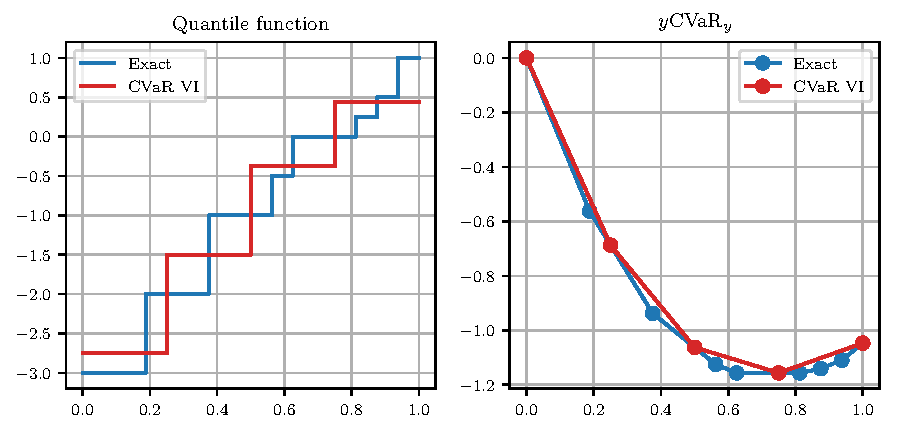
\includegraphics[width=\linewidth]{../gfx/cvar_visualized.pdf}
\caption{Comparison of a discrete distribution and it's approximation according to the CVaR linear interpolation operator.}
\label{fig:cvarvisual}
\end{figure}

\subsection{CVaR Computation via Quantile Representation}

We propose the following procedure: instead of using linear programming for the CVaR computation, we use the underlying distributions represented by the $\alpha \cvar_\alpha$ function to compute CVaR at each atom. The general steps of the computation are as follows

%\begin{algorithm}[h]
%\caption{Value Iteration via Quantile Representation}
%\label{alg:fastvi}
%\begin{enumerate}
%\item transform $y \cvar_y$ of each possible state transition to a discrete probability distribution function using \eqnref{varcvarderivation}
%\item combine these to to a distribution representing the full state-action distribution
%\item compute $y \cvar_y$ for all atoms using \eqnref{varcvarintegration}
%\end{enumerate}
%\end{algorithm}

\begin{enumerate}
\item transform $y \cvar_y$ of each possible state transition to a discrete probability distribution using \eqnref{varcvarderivation}
\item combine these to to a distribution representing the full state-action distribution
\item compute $y \cvar_y$ for all atoms using \eqnref{varcvarintegration}
\end{enumerate}
See \figref{cvarcomputation} for a visualization of the procedure. 
\\
Note that this procedure is linear for discrete distributions.
\begin{figure}
\center
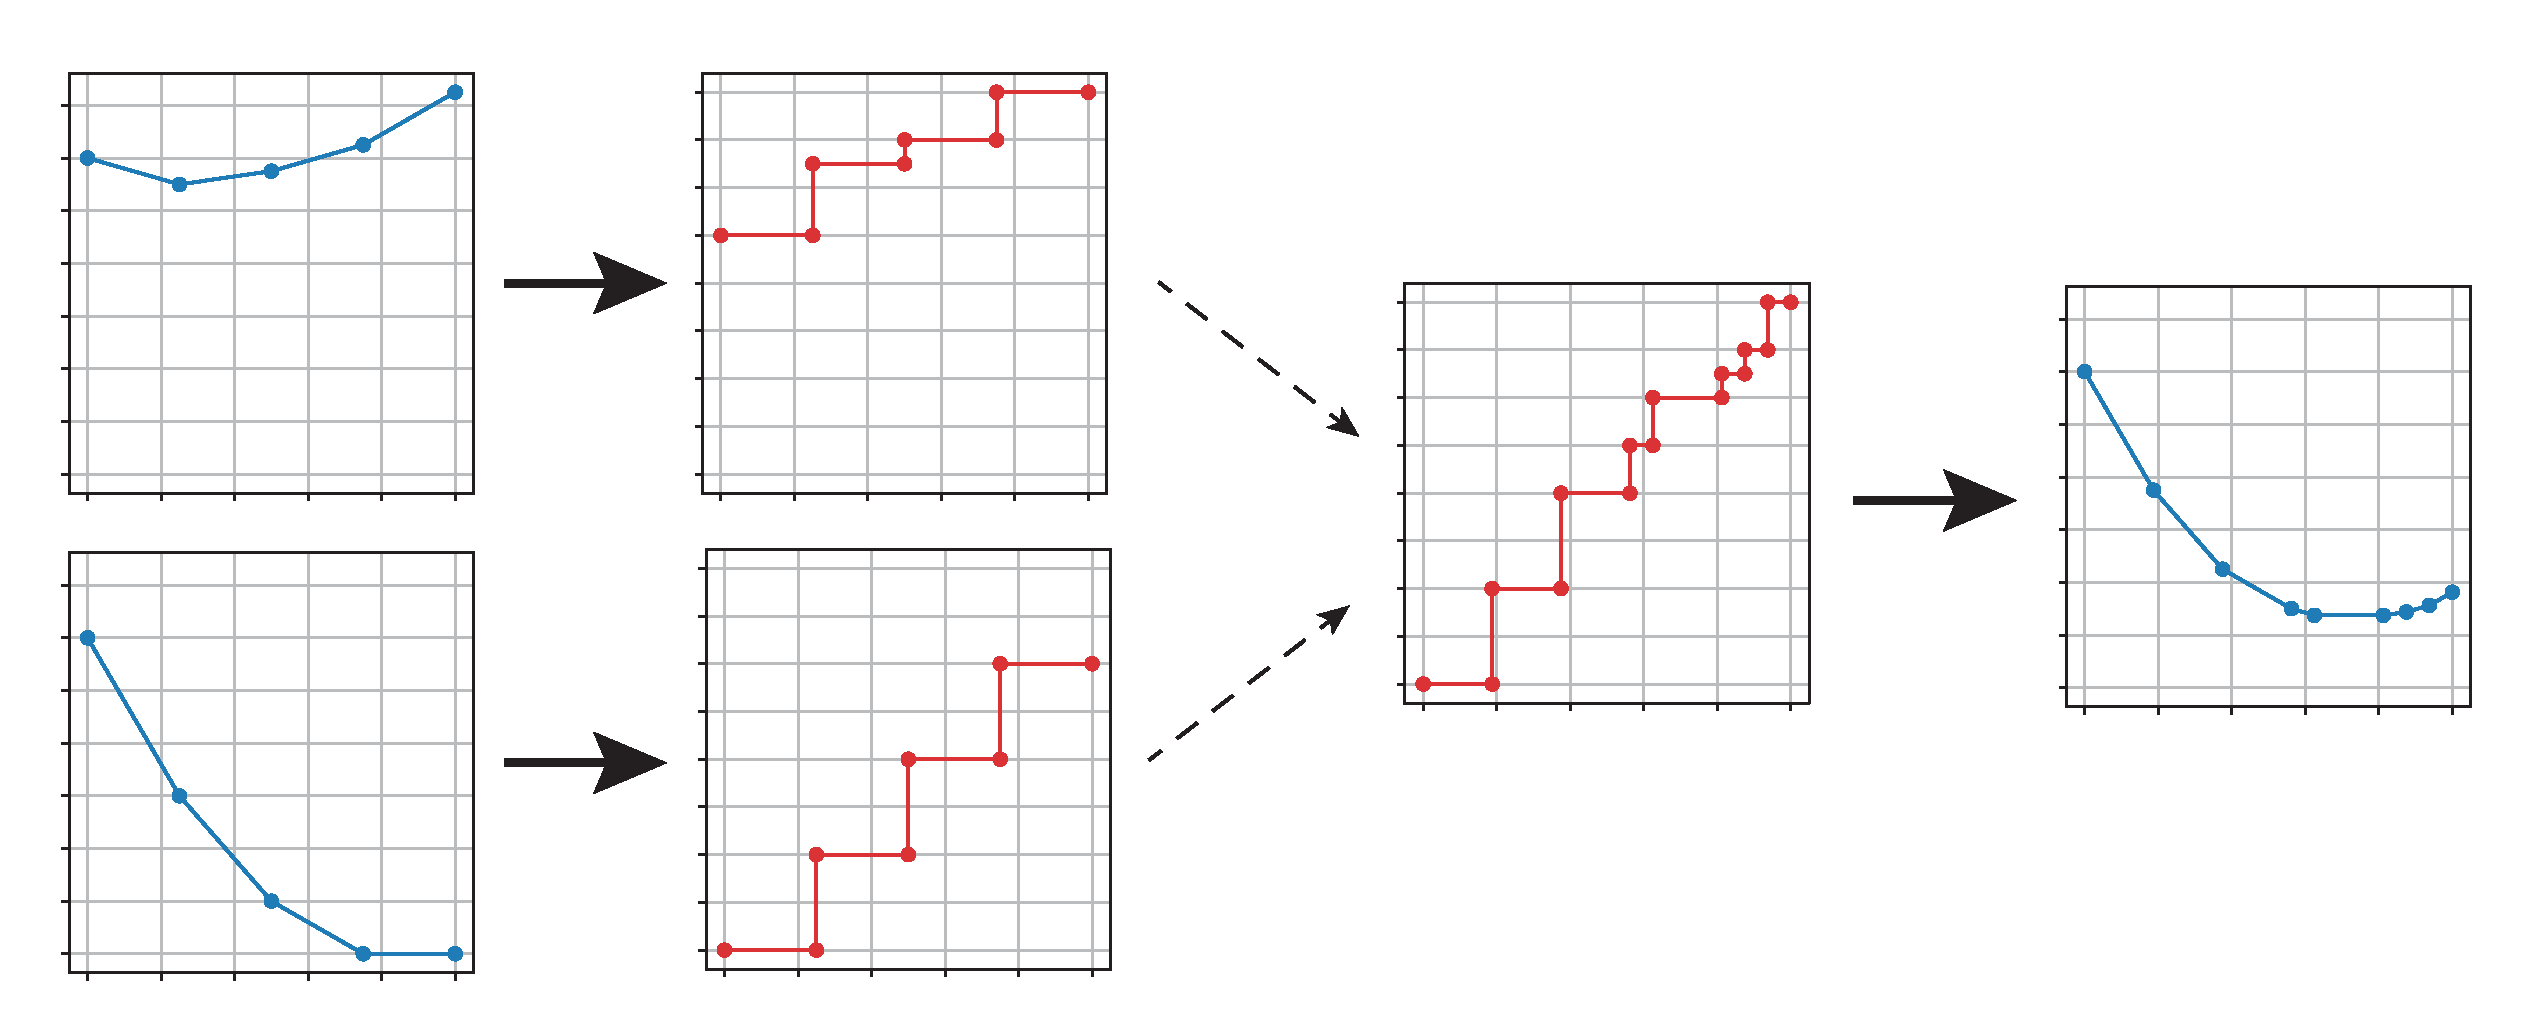
\includegraphics[width=\linewidth]{../gfx/cvar_vi_conversion.pdf}
\caption{Visualization of the CVaR computation for a single state and action with two transition states. Thick arrows represent the conversion between $\ycvary$ and the quantile function.}
\label{fig:cvarcomputation}
\end{figure}
To show the correctness of this approach, we formulate it as a solution to the problem \eqnref{cvardecomp}. Note that we skip the reward and gamma scaling for readability's sake. The extension to the bellman operator is trivial.

\subsection{$\xi$-computation}

Similarly to \thmref{optimalpolicy}, we need a way to compute the $y_{k+1}=y_{k}\xi^*(x_k)$ to extract the optimal policy. We compute $\xi^*(x_k)$ by using the following intuition: $y_{k+1}$ is the portion of $Z(x_{k+1})$ that is present in $\cvar_{y_k}(Z(x_k))$. In the continuous case, it is the probability in $Z(x_{k+1})$ before the $\var_{y_k}(Z(x_k))$ as we show bellow.

\begin{theorem}
Let $x_1', x_2'$ be two states reachable from state $x$ in a single transition. Let the cumulative distribution functions of the state's underlying distributions $Z(x_1'), Z(x_2)$ be strictly increasing with unbounded support.
Then the solution to minimization problem \eqnref{cvardecomp} can be computed setting
\begin{equation}\label{eqn:xi-claim}
\xi ( x_i' ) = \dfrac{F_{x_i'}(F^{-1}_x(\alpha))}{\alpha} 
\end{equation}
\end{theorem}



\subsection{Q-learning}\label{sec:qlearning}

Q-learning (\cite{watkins1992q}) is an important off-policy temporal difference control algorithm, that works by repeatedly updating the $Q$ value estimate according to the sampled rewards and states using a moving exponential average.
\begin{equation}
\begin{split}
&Q_{t+1}(x, a) = (1-\beta)Q_{t}(x, a) + \beta\bsquare{r + \gamma \max_{a'} Q_t(x', a')}\\
&x' \sim p(\cdot|x, a)
\end{split}
\end{equation}
Here $Q$ is an estimate of the optimal action-value function and $\beta$ is the learning rate. The order of the visited states is unimportant, as long as all reachable states are updated infinitely often and the learning rate meets a standard condition used in stochastic approximation.
\begin{equation}\label{eqn:beta}
\sum_{t=0}^\infty \beta_t = \infty  \quad \sum_{t=0}^\infty \beta_t^2 < \infty\\
\end{equation}
See \cite{jaakkola1994convergence} for details.

\subsection{CVaR estimation}\label{sec:cvarestimation}

Before formulating a CVaR version of Q-learning, we must first talk about simply \emph{estimating} CVaR, as it is not as straightforward as the estimation of expected value.

Let us remind ourselves of the primal definition of CVaR \eqnref{cvarprimal}:
\begin{equation*}
\cvar_\alpha(Z)=
\max_s\left\lbrace \dfrac{1}{\alpha}\expect
\left[ (Z-s)^-\right] + s  \right\rbrace 
\end{equation*}
If we knew the exact $s^*=\var_\alpha$, we could estimate the CVaR as a simple expectation of the $\dfrac{1}{\alpha}(Z-s^*)^-+s^*$ function. As we do not know this value in advance, a common approach is to first approximate $\var_\alpha$ from data, then use this estimate to compute it's $\cvar_\alpha$. This is usually done with a full data vector, requiring the whole data history to be saved in memory.

When dealing with reinforcement learning, we would like to store our current estimate as a scalar instead. This requires finding a recursive expression whose expectation is the CVaR value. Fortunately, similar methods have been thoroughly investigated in the stochastic approximation literature by \cite{robbins1951stochastic}.

The RM theorem has also been applied directly to CVaR estimation by \cite{bardou2009recursive}, who used it to formulate a recursive importance sampling procedure useful for estimating CVaR of long-tailed distributions.

First let us describe the method for a one step estimation, meaning we sample values (or rewards in our case) $r$ from some distribution and our goal is to estimate CVaR at a given confidence level $\alpha$. The procedure requires us to maintain two separate estimates $V$ and $C$, being our VaR and CVaR estimates respectively.
\begin{align}
V_{t+1} &= V_{t} + \beta \bsquare{1-\dfrac{1}{\alpha}\mathbbm{1}_{(V_t \ge r)}}\label{eqn:varestimate}\\
C_{t+1} &= (1-\beta)C_t + \beta \bsquare{V_t + \dfrac{1}{\alpha}(r-V_t)^-}\label{eqn:cvarestimate}
\end{align}

An observant reader may recognize a standard equation for quantile estimation in equation \eqnref{varestimate} (see e.g. \cite{koenker2001quantile} for more information on quantile estimation/regression) and equation \eqnref{cvarestimate} is also quite intuitive, representing the moving exponential average of the primal CVaR definition \eqnref{cvarprimal}. The estimations are proven to converge, given the usual requirements on the learning rate \eqnref{beta} \cite{bardou2009recursive}.


\section{CVaR Q-learning}\label{sec:qcvar}

We now extend the previously established CVaR value iteration and combine it with the recursive CVaR estimation techniques to formulate a new algorithm we call CVaR Q-learning.
\subsection{Temporal Difference update}
We first define two separate values for each state, action and atom $V, C: \cX\times\cA\times\cY\to\real$ where $C(x, a, y)$ represents $\cvar_y(Z(x, a))$ of the distribution, similar to the definition \eqnref{cdef}. $V(x, a, y)$ represents the one-step $\var_y$ estimate, or the estimate of the $y-$quantile of a distribution recovered from $\cvar_y$ by Lemma \ref{thm:varcvarconnection}.

A key to any TD algorithm is it's update rule. The CVaR TD update rule extends the improved VI procedure and we present the full rule in \algref{cvartd}. 

Let us now go through the algorithm and compare the two versions. We first construct a new CVaR (line \ref{alg:cvartd:1}) by greedily selecting actions that yield the highest CVaR for each atom. This step is somewhat skipped in the VI process since we are not working with action-value functions. These values are then transformed to their underlying distributions (line \ref{alg:cvartd:2}) and used to generate 'samples' $v$ from this distribution. Quotes are used here since we know the distributions and do not have to actually sample - instead we use the quantile values proportionally to their probabilities. Similar technique has been used to minimize the Wasserstein distance of a learned distribution by \cite{dabney2017distributional}.

If the atoms aren't uniform, we perform basic importance sampling (line \label{alg:cvartd:3}) to weight each 'sample' according to it's probability. Finally, these ***samples*** are used to update the respective VaR and CVaR estimates.


\begin{algorithm}[H]
\caption{CVaR TD update}
\begin{algorithmic}[1]\label{alg:cvartd}

    \STATE \textbf{input:} $x, a, x', r$
    
    \FOR{each $y_i$ }
	\STATE $C(x', y_i) = \max_{a'} C(x', a', y_i)$ \label{alg:cvartd:1}
	\ENDFOR
	
	\STATE todo: introduce notation to C, v \label{alg:cvartd:2}

	\FOR{each $v$, $y_i$}
	\STATE $\beta_i = \beta (y_i-y_{i-1})$  \label{alg:cvartd:3}
	\STATE $V(x, a, y_i) = V(x, a, y_i) + \beta_i \bsquare{1 - \dfrac{1}{y_i}\mathbbm{1}_{(V(x, a, y_i) \ge r+\gamma v)}}$  \label{alg:cvartd:4}
	\STATE $C(x, a, y_i) = (1-\beta_i)C(x, a, y_i) + \beta_i \bsquare{V(x, a, y_i) + \dfrac{1}{y_i}\bround{r+\gamma v - V(x, a, y_i)}^-}$  \label{alg:cvartd:5}
	\ENDFOR
	
\end{algorithmic}
\end{algorithm}


\section{Convergence}
The main problem faced here is one of convergence. We would like to know if the proposed Q-learning algorithm converges.

Positive results: 1) The interpolated VI is a contraction, 2) the 1-step VaR-CVaR estimation converges w.p. 1(unclear if it only converges for continuous distributions)

Unclear: does the whole procedure converge?


\bibliographystyle{unsrt}
\bibliography{../Bibliography.bib}

\end{document}




